\documentclass[1p]{elsarticle_modified}
%\bibliographystyle{elsarticle-num}

%\usepackage[colorlinks]{hyperref}
%\usepackage{abbrmath_seonhwa} %\Abb, \Ascr, \Acal ,\Abf, \Afrak
\usepackage{amsfonts}
\usepackage{amssymb}
\usepackage{amsmath}
\usepackage{amsthm}
\usepackage{scalefnt}
\usepackage{amsbsy}
\usepackage{kotex}
\usepackage{caption}
\usepackage{subfig}
\usepackage{color}
\usepackage{graphicx}
\usepackage{xcolor} %% white, black, red, green, blue, cyan, magenta, yellow
\usepackage{float}
\usepackage{setspace}
\usepackage{hyperref}

\usepackage{tikz}
\usetikzlibrary{arrows}

\usepackage{multirow}
\usepackage{array} % fixed length table
\usepackage{hhline}

%%%%%%%%%%%%%%%%%%%%%
\makeatletter
\renewcommand*\env@matrix[1][\arraystretch]{%
	\edef\arraystretch{#1}%
	\hskip -\arraycolsep
	\let\@ifnextchar\new@ifnextchar
	\array{*\c@MaxMatrixCols c}}
\makeatother %https://tex.stackexchange.com/questions/14071/how-can-i-increase-the-line-spacing-in-a-matrix
%%%%%%%%%%%%%%%

\usepackage[normalem]{ulem}

\newcommand{\msout}[1]{\ifmmode\text{\sout{\ensuremath{#1}}}\else\sout{#1}\fi}
%SOURCE: \msout is \stkout macro in https://tex.stackexchange.com/questions/20609/strikeout-in-math-mode

\newcommand{\cancel}[1]{
	\ifmmode
	{\color{red}\msout{#1}}
	\else
	{\color{red}\sout{#1}}
	\fi
}

\newcommand{\add}[1]{
	{\color{blue}\uwave{#1}}
}

\newcommand{\replace}[2]{
	\ifmmode
	{\color{red}\msout{#1}}{\color{blue}\uwave{#2}}
	\else
	{\color{red}\sout{#1}}{\color{blue}\uwave{#2}}
	\fi
}

\newcommand{\Sol}{\mathcal{S}} %segment
\newcommand{\D}{D} %diagram
\newcommand{\A}{\mathcal{A}} %arc


%%%%%%%%%%%%%%%%%%%%%%%%%%%%%5 test

\def\sl{\operatorname{\textup{SL}}(2,\Cbb)}
\def\psl{\operatorname{\textup{PSL}}(2,\Cbb)}
\def\quan{\mkern 1mu \triangleright \mkern 1mu}

\theoremstyle{definition}
\newtheorem{thm}{Theorem}[section]
\newtheorem{prop}[thm]{Proposition}
\newtheorem{lem}[thm]{Lemma}
\newtheorem{ques}[thm]{Question}
\newtheorem{cor}[thm]{Corollary}
\newtheorem{defn}[thm]{Definition}
\newtheorem{exam}[thm]{Example}
\newtheorem{rmk}[thm]{Remark}
\newtheorem{alg}[thm]{Algorithm}

\newcommand{\I}{\sqrt{-1}}
\begin{document}

%\begin{frontmatter}
%
%\title{Boundary parabolic representations of knots up to 8 crossings}
%
%%% Group authors per affiliation:
%\author{Yunhi Cho} 
%\address{Department of Mathematics, University of Seoul, Seoul, Korea}
%\ead{yhcho@uos.ac.kr}
%
%
%\author{Seonhwa Kim} %\fnref{s_kim}}
%\address{Center for Geometry and Physics, Institute for Basic Science, Pohang, 37673, Korea}
%\ead{ryeona17@ibs.re.kr}
%
%\author{Hyuk Kim}
%\address{Department of Mathematical Sciences, Seoul National University, Seoul 08826, Korea}
%\ead{hyukkim@snu.ac.kr}
%
%\author{Seokbeom Yoon}
%\address{Department of Mathematical Sciences, Seoul National University, Seoul, 08826,  Korea}
%\ead{sbyoon15@snu.ac.kr}
%
%\begin{abstract}
%We find all boundary parabolic representation of knots up to 8 crossings.
%
%\end{abstract}
%\begin{keyword}
%    \MSC[2010] 57M25 
%\end{keyword}
%
%\end{frontmatter}

%\linenumbers
%\tableofcontents
%
\newcommand\colored[1]{\textcolor{white}{\rule[-0.35ex]{0.8em}{1.4ex}}\kern-0.8em\color{red} #1}%
%\newcommand\colored[1]{\textcolor{white}{ #1}\kern-2.17ex	\textcolor{white}{ #1}\kern-1.81ex	\textcolor{white}{ #1}\kern-2.15ex\color{red}#1	}

{\Large $\underline{12n_{0359}~(K12n_{0359})}$}

\setlength{\tabcolsep}{10pt}
\renewcommand{\arraystretch}{1.6}
\vspace{1cm}\begin{tabular}{m{100pt}>{\centering\arraybackslash}m{274pt}}
\multirow{5}{120pt}{
	\centering
	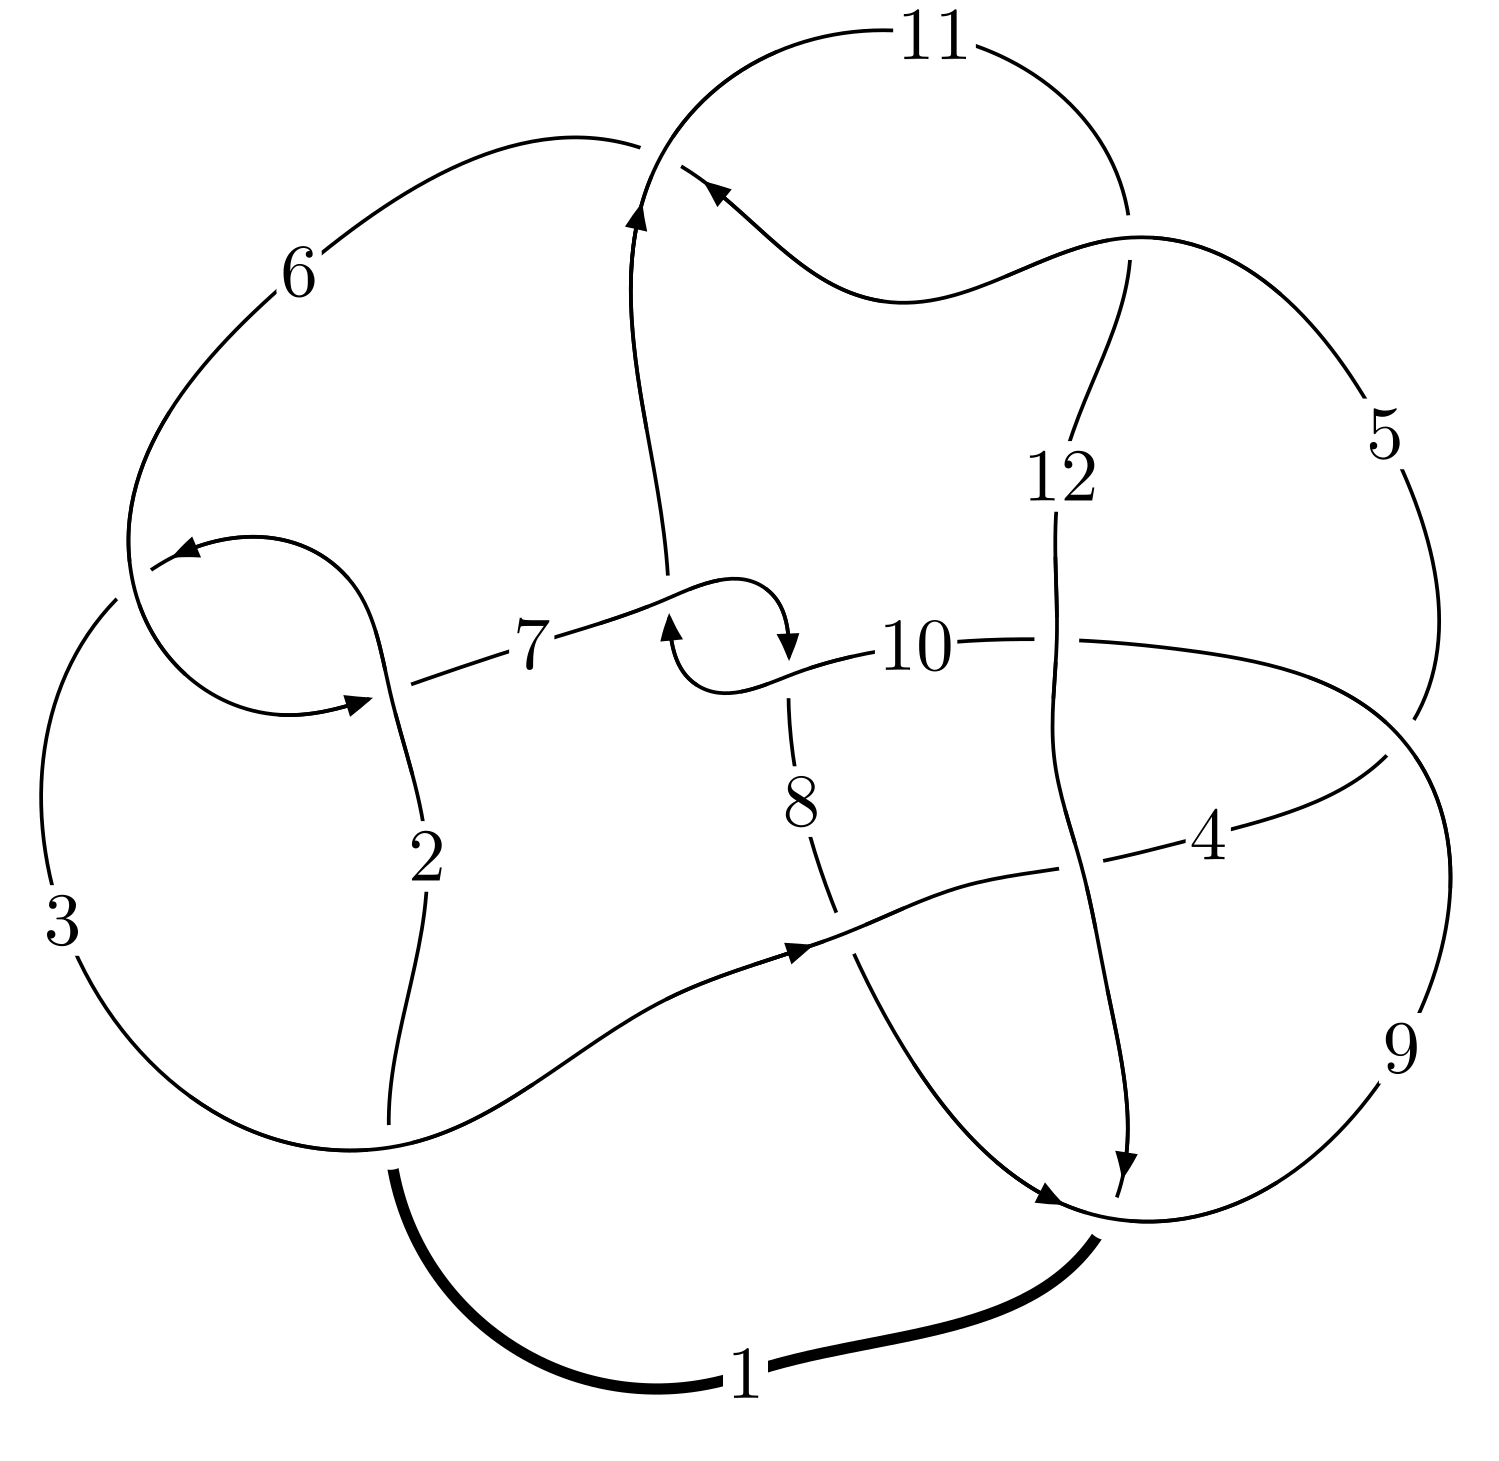
\includegraphics[width=112pt]{../../../GIT/diagram.site/Diagrams/png/2448_12n_0359.png}\\
\ \ \ A knot diagram\footnotemark}&
\allowdisplaybreaks
\textbf{Linearized knot diagam} \\
\cline{2-2}
 &
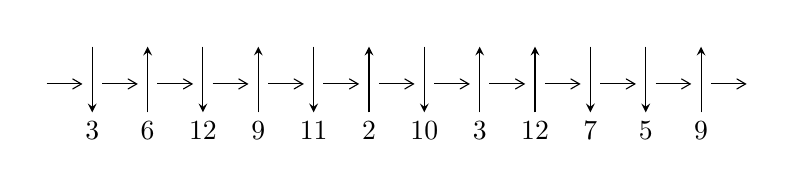
\begin{tikzpicture}[x=20pt, y=17pt]
	% nodes
	\node (C0) at (0, 0) {};
	\node (C1) at (1, 0) {};
	\node (C1U) at (1, +1) {};
	\node (C1D) at (1, -1) {3};

	\node (C2) at (2, 0) {};
	\node (C2U) at (2, +1) {};
	\node (C2D) at (2, -1) {6};

	\node (C3) at (3, 0) {};
	\node (C3U) at (3, +1) {};
	\node (C3D) at (3, -1) {12};

	\node (C4) at (4, 0) {};
	\node (C4U) at (4, +1) {};
	\node (C4D) at (4, -1) {9};

	\node (C5) at (5, 0) {};
	\node (C5U) at (5, +1) {};
	\node (C5D) at (5, -1) {11};

	\node (C6) at (6, 0) {};
	\node (C6U) at (6, +1) {};
	\node (C6D) at (6, -1) {2};

	\node (C7) at (7, 0) {};
	\node (C7U) at (7, +1) {};
	\node (C7D) at (7, -1) {10};

	\node (C8) at (8, 0) {};
	\node (C8U) at (8, +1) {};
	\node (C8D) at (8, -1) {3};

	\node (C9) at (9, 0) {};
	\node (C9U) at (9, +1) {};
	\node (C9D) at (9, -1) {12};

	\node (C10) at (10, 0) {};
	\node (C10U) at (10, +1) {};
	\node (C10D) at (10, -1) {7};

	\node (C11) at (11, 0) {};
	\node (C11U) at (11, +1) {};
	\node (C11D) at (11, -1) {5};

	\node (C12) at (12, 0) {};
	\node (C12U) at (12, +1) {};
	\node (C12D) at (12, -1) {9};
	\node (C13) at (13, 0) {};

	% arrows
	\draw[->,>={angle 60}]
	(C0) edge (C1) (C1) edge (C2) (C2) edge (C3) (C3) edge (C4) (C4) edge (C5) (C5) edge (C6) (C6) edge (C7) (C7) edge (C8) (C8) edge (C9) (C9) edge (C10) (C10) edge (C11) (C11) edge (C12) (C12) edge (C13) ;	\draw[->,>=stealth]
	(C1U) edge (C1D) (C2D) edge (C2U) (C3U) edge (C3D) (C4D) edge (C4U) (C5U) edge (C5D) (C6D) edge (C6U) (C7U) edge (C7D) (C8D) edge (C8U) (C9D) edge (C9U) (C10U) edge (C10D) (C11U) edge (C11D) (C12D) edge (C12U) ;
	\end{tikzpicture} \\
\hhline{~~} \\& 
\textbf{Solving Sequence} \\ \cline{2-2} 
 &
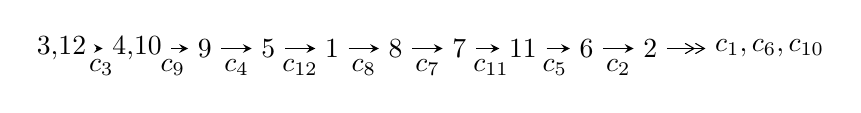
\begin{tikzpicture}[x=23pt, y=7pt]
	% node
	\node (A0) at (-1/8, 0) {3,12};
	\node (A1) at (17/16, 0) {4,10};
	\node (A2) at (17/8, 0) {9};
	\node (A3) at (25/8, 0) {5};
	\node (A4) at (33/8, 0) {1};
	\node (A5) at (41/8, 0) {8};
	\node (A6) at (49/8, 0) {7};
	\node (A7) at (57/8, 0) {11};
	\node (A8) at (65/8, 0) {6};
	\node (A9) at (73/8, 0) {2};
	\node (C1) at (1/2, -1) {$c_{3}$};
	\node (C2) at (13/8, -1) {$c_{9}$};
	\node (C3) at (21/8, -1) {$c_{4}$};
	\node (C4) at (29/8, -1) {$c_{12}$};
	\node (C5) at (37/8, -1) {$c_{8}$};
	\node (C6) at (45/8, -1) {$c_{7}$};
	\node (C7) at (53/8, -1) {$c_{11}$};
	\node (C8) at (61/8, -1) {$c_{5}$};
	\node (C9) at (69/8, -1) {$c_{2}$};
	\node (A10) at (11, 0) {$c_{1},c_{6},c_{10}$};

	% edge
	\draw[->,>=stealth]	
	(A0) edge (A1) (A1) edge (A2) (A2) edge (A3) (A3) edge (A4) (A4) edge (A5) (A5) edge (A6) (A6) edge (A7) (A7) edge (A8) (A8) edge (A9) ;
	\draw[->>,>={angle 60}]	
	(A9) edge (A10);
\end{tikzpicture} \\ 

\end{tabular} \\

\footnotetext{
The image of knot diagram is generated by the software ``\textbf{Draw programme}" developed by Andrew Bartholomew(\url{http://www.layer8.co.uk/maths/draw/index.htm\#Running-draw}), where we modified some parts for our purpose(\url{https://github.com/CATsTAILs/LinksPainter}).
}\phantom \\ \newline 
\centering \textbf{Ideals for irreducible components\footnotemark of $X_{\text{par}}$} 
 
\begin{align*}
I^u_{1}&=\langle 
-1.47058\times10^{201} u^{51}+5.71881\times10^{201} u^{50}+\cdots+6.09460\times10^{202} b+1.54791\times10^{203},\\
\phantom{I^u_{1}}&\phantom{= \langle  }-1.76593\times10^{202} u^{51}+1.24322\times10^{204} u^{50}+\cdots+2.49879\times10^{204} a+8.25019\times10^{206},\\
\phantom{I^u_{1}}&\phantom{= \langle  }u^{52}-3 u^{51}+\cdots+774 u+41\rangle \\
I^u_{2}&=\langle 
-352794218079 u^{17}-1984503379263 u^{16}+\cdots+27696360721 b-8429306818513,\\
\phantom{I^u_{2}}&\phantom{= \langle  }-9258892608982 u^{17}-56236696433763 u^{16}+\cdots+470838132257 a-283519838364447,\\
\phantom{I^u_{2}}&\phantom{= \langle  }u^{18}+6 u^{17}+\cdots+137 u+17\rangle \\
\\
\end{align*}
\raggedright * 2 irreducible components of $\dim_{\mathbb{C}}=0$, with total 70 representations.\\
\footnotetext{All coefficients of polynomials are rational numbers. But the coefficients are sometimes approximated in decimal forms when there is not enough margin.}
\newpage
\renewcommand{\arraystretch}{1}
\centering \section*{I. $I^u_{1}= \langle -1.47\times10^{201} u^{51}+5.72\times10^{201} u^{50}+\cdots+6.09\times10^{202} b+1.55\times10^{203},\;-1.77\times10^{202} u^{51}+1.24\times10^{204} u^{50}+\cdots+2.50\times10^{204} a+8.25\times10^{206},\;u^{52}-3 u^{51}+\cdots+774 u+41 \rangle$}
\flushleft \textbf{(i) Arc colorings}\\
\begin{tabular}{m{7pt} m{180pt} m{7pt} m{180pt} }
\flushright $a_{3}=$&$\begin{pmatrix}1\\0\end{pmatrix}$ \\
\flushright $a_{12}=$&$\begin{pmatrix}0\\u\end{pmatrix}$ \\
\flushright $a_{4}=$&$\begin{pmatrix}1\\u^2\end{pmatrix}$ \\
\flushright $a_{10}=$&$\begin{pmatrix}0.00706714 u^{51}-0.497531 u^{50}+\cdots-4176.94 u-330.168\\0.0241292 u^{51}-0.0938340 u^{50}+\cdots-43.0144 u-2.53980\end{pmatrix}$ \\
\flushright $a_{9}=$&$\begin{pmatrix}0.00706714 u^{51}-0.497531 u^{50}+\cdots-4176.94 u-330.168\\0.197950 u^{51}-0.650977 u^{50}+\cdots+325.375 u+16.9897\end{pmatrix}$ \\
\flushright $a_{5}=$&$\begin{pmatrix}3.73750 u^{51}-11.7980 u^{50}+\cdots+9454.68 u+541.305\\0.193063 u^{51}-0.579335 u^{50}+\cdots+677.585 u+43.3523\end{pmatrix}$ \\
\flushright $a_{1}=$&$\begin{pmatrix}-2.42736 u^{51}+7.50252 u^{50}+\cdots-7583.02 u-470.483\\0.650781 u^{51}-1.98369 u^{50}+\cdots+2282.43 u+144.200\end{pmatrix}$ \\
\flushright $a_{8}=$&$\begin{pmatrix}-0.190883 u^{51}+0.153446 u^{50}+\cdots-4502.31 u-347.158\\0.197950 u^{51}-0.650977 u^{50}+\cdots+325.375 u+16.9897\end{pmatrix}$ \\
\flushright $a_{7}=$&$\begin{pmatrix}-3.76231 u^{51}+12.0301 u^{50}+\cdots-8407.16 u-464.145\\0.726083 u^{51}-2.30029 u^{50}+\cdots+1789.52 u+100.639\end{pmatrix}$ \\
\flushright $a_{11}=$&$\begin{pmatrix}2.24745 u^{51}-6.98939 u^{50}+\cdots+6618.23 u+408.458\\-0.635359 u^{51}+1.80797 u^{50}+\cdots-3338.50 u-227.183\end{pmatrix}$ \\
\flushright $a_{6}=$&$\begin{pmatrix}-0.815911 u^{51}+2.78119 u^{50}+\cdots-191.619 u+36.3758\\-0.365167 u^{51}+1.04144 u^{50}+\cdots-1859.62 u-126.481\end{pmatrix}$ \\
\flushright $a_{2}=$&$\begin{pmatrix}-3.07815 u^{51}+9.48621 u^{50}+\cdots-9865.45 u-614.683\\0.650781 u^{51}-1.98369 u^{50}+\cdots+2282.43 u+144.200\end{pmatrix}$\\&\end{tabular}
\flushleft \textbf{(ii) Obstruction class $= -1$}\\~\\
\flushleft \textbf{(iii) Cusp Shapes $= -2.01660 u^{51}+5.78735 u^{50}+\cdots-10137.6 u-684.151$}\\~\\
\newpage\renewcommand{\arraystretch}{1}
\flushleft \textbf{(iv) u-Polynomials at the component}\newline \\
\begin{tabular}{m{50pt}|m{274pt}}
Crossings & \hspace{64pt}u-Polynomials at each crossing \\
\hline $$\begin{aligned}c_{1}\end{aligned}$$&$\begin{aligned}
&u^{52}+29 u^{51}+\cdots+1305 u+49
\end{aligned}$\\
\hline $$\begin{aligned}c_{2},c_{6}\end{aligned}$$&$\begin{aligned}
&u^{52}-3 u^{51}+\cdots-33 u+7
\end{aligned}$\\
\hline $$\begin{aligned}c_{3}\end{aligned}$$&$\begin{aligned}
&u^{52}-3 u^{51}+\cdots+774 u+41
\end{aligned}$\\
\hline $$\begin{aligned}c_{4}\end{aligned}$$&$\begin{aligned}
&u^{52}+u^{51}+\cdots-6854 u+3421
\end{aligned}$\\
\hline $$\begin{aligned}c_{5},c_{11}\end{aligned}$$&$\begin{aligned}
&u^{52}+u^{51}+\cdots+67 u+173
\end{aligned}$\\
\hline $$\begin{aligned}c_{7},c_{10}\end{aligned}$$&$\begin{aligned}
&u^{52}-5 u^{51}+\cdots-175 u+43
\end{aligned}$\\
\hline $$\begin{aligned}c_{8}\end{aligned}$$&$\begin{aligned}
&u^{52}- u^{51}+\cdots+35897 u+98677
\end{aligned}$\\
\hline $$\begin{aligned}c_{9},c_{12}\end{aligned}$$&$\begin{aligned}
&u^{52}+u^{51}+\cdots-164 u+14
\end{aligned}$\\
\hline
\end{tabular}\\~\\
\newpage\renewcommand{\arraystretch}{1}
\flushleft \textbf{(v) Riley Polynomials at the component}\newline \\
\begin{tabular}{m{50pt}|m{274pt}}
Crossings & \hspace{64pt}Riley Polynomials at each crossing \\
\hline $$\begin{aligned}c_{1}\end{aligned}$$&$\begin{aligned}
&y^{52}+y^{51}+\cdots-11839 y+2401
\end{aligned}$\\
\hline $$\begin{aligned}c_{2},c_{6}\end{aligned}$$&$\begin{aligned}
&y^{52}+29 y^{51}+\cdots+1305 y+49
\end{aligned}$\\
\hline $$\begin{aligned}c_{3}\end{aligned}$$&$\begin{aligned}
&y^{52}-91 y^{51}+\cdots-17778 y+1681
\end{aligned}$\\
\hline $$\begin{aligned}c_{4}\end{aligned}$$&$\begin{aligned}
&y^{52}+65 y^{51}+\cdots+435342632 y+11703241
\end{aligned}$\\
\hline $$\begin{aligned}c_{5},c_{11}\end{aligned}$$&$\begin{aligned}
&y^{52}+47 y^{51}+\cdots+156055 y+29929
\end{aligned}$\\
\hline $$\begin{aligned}c_{7},c_{10}\end{aligned}$$&$\begin{aligned}
&y^{52}+21 y^{51}+\cdots+50043 y+1849
\end{aligned}$\\
\hline $$\begin{aligned}c_{8}\end{aligned}$$&$\begin{aligned}
&y^{52}+71 y^{51}+\cdots+159369402631 y+9737150329
\end{aligned}$\\
\hline $$\begin{aligned}c_{9},c_{12}\end{aligned}$$&$\begin{aligned}
&y^{52}+65 y^{51}+\cdots+1188 y+196
\end{aligned}$\\
\hline
\end{tabular}\\~\\
\newpage\flushleft \textbf{(vi) Complex Volumes and Cusp Shapes}
$$\begin{array}{c|c|c}  
\text{Solutions to }I^u_{1}& \I (\text{vol} + \sqrt{-1}CS) & \text{Cusp shape}\\
 \hline 
\begin{aligned}
u &= -0.847196 + 0.544439 I \\
a &= \phantom{-}0.821121 - 1.049870 I \\
b &= \phantom{-}1.283350 + 0.463702 I\end{aligned}
 & \phantom{-}2.14411 + 0.25670 I & \phantom{-0.000000 } 0 \\ \hline\begin{aligned}
u &= -0.847196 - 0.544439 I \\
a &= \phantom{-}0.821121 + 1.049870 I \\
b &= \phantom{-}1.283350 - 0.463702 I\end{aligned}
 & \phantom{-}2.14411 - 0.25670 I & \phantom{-0.000000 } 0 \\ \hline\begin{aligned}
u &= -0.633779 + 0.695586 I \\
a &= -0.465169 + 0.186673 I \\
b &= -0.777699 + 0.134617 I\end{aligned}
 & \phantom{-}0.20861 + 2.21635 I & \phantom{-0.000000 } 0 \\ \hline\begin{aligned}
u &= -0.633779 - 0.695586 I \\
a &= -0.465169 - 0.186673 I \\
b &= -0.777699 - 0.134617 I\end{aligned}
 & \phantom{-}0.20861 - 2.21635 I & \phantom{-0.000000 } 0 \\ \hline\begin{aligned}
u &= -1.050210 + 0.243025 I \\
a &= -1.018580 + 0.716714 I \\
b &= -0.003518 - 0.905590 I\end{aligned}
 & \phantom{-}1.62405 + 1.56252 I & \phantom{-0.000000 } 0 \\ \hline\begin{aligned}
u &= -1.050210 - 0.243025 I \\
a &= -1.018580 - 0.716714 I \\
b &= -0.003518 + 0.905590 I\end{aligned}
 & \phantom{-}1.62405 - 1.56252 I & \phantom{-0.000000 } 0 \\ \hline\begin{aligned}
u &= \phantom{-}0.244644 + 0.877276 I \\
a &= -1.323870 - 0.306984 I \\
b &= -1.55896 - 0.12562 I\end{aligned}
 & \phantom{-}1.74102 + 5.91393 I & \phantom{-0.000000 } 0 \\ \hline\begin{aligned}
u &= \phantom{-}0.244644 - 0.877276 I \\
a &= -1.323870 + 0.306984 I \\
b &= -1.55896 + 0.12562 I\end{aligned}
 & \phantom{-}1.74102 - 5.91393 I & \phantom{-0.000000 } 0 \\ \hline\begin{aligned}
u &= \phantom{-}0.025679 + 0.905219 I \\
a &= \phantom{-}0.551984 + 0.188120 I \\
b &= \phantom{-}0.917186 + 0.799077 I\end{aligned}
 & \phantom{-}0.33243 + 2.42561 I & \phantom{-0.000000 } 0 \\ \hline\begin{aligned}
u &= \phantom{-}0.025679 - 0.905219 I \\
a &= \phantom{-}0.551984 - 0.188120 I \\
b &= \phantom{-}0.917186 - 0.799077 I\end{aligned}
 & \phantom{-}0.33243 - 2.42561 I & \phantom{-0.000000 } 0\\
 \hline 
 \end{array}$$\newpage$$\begin{array}{c|c|c}  
\text{Solutions to }I^u_{1}& \I (\text{vol} + \sqrt{-1}CS) & \text{Cusp shape}\\
 \hline 
\begin{aligned}
u &= \phantom{-}0.765182 + 1.001930 I \\
a &= \phantom{-}0.914709 + 0.294749 I \\
b &= -0.309410 - 0.681136 I\end{aligned}
 & \phantom{-}5.54999 + 1.24202 I & \phantom{-0.000000 } 0 \\ \hline\begin{aligned}
u &= \phantom{-}0.765182 - 1.001930 I \\
a &= \phantom{-}0.914709 - 0.294749 I \\
b &= -0.309410 + 0.681136 I\end{aligned}
 & \phantom{-}5.54999 - 1.24202 I & \phantom{-0.000000 } 0 \\ \hline\begin{aligned}
u &= \phantom{-}0.248997 + 1.272460 I \\
a &= \phantom{-}0.245962 + 0.003913 I \\
b &= -0.696361 - 0.656099 I\end{aligned}
 & \phantom{-}7.59032 + 0.63287 I & \phantom{-0.000000 } 0 \\ \hline\begin{aligned}
u &= \phantom{-}0.248997 - 1.272460 I \\
a &= \phantom{-}0.245962 - 0.003913 I \\
b &= -0.696361 + 0.656099 I\end{aligned}
 & \phantom{-}7.59032 - 0.63287 I & \phantom{-0.000000 } 0 \\ \hline\begin{aligned}
u &= -0.638428 + 1.232980 I \\
a &= -0.642920 + 0.541264 I \\
b &= \phantom{-}0.385485 - 0.613568 I\end{aligned}
 & \phantom{-}2.65578 - 3.46508 I & \phantom{-0.000000 } 0 \\ \hline\begin{aligned}
u &= -0.638428 - 1.232980 I \\
a &= -0.642920 - 0.541264 I \\
b &= \phantom{-}0.385485 + 0.613568 I\end{aligned}
 & \phantom{-}2.65578 + 3.46508 I & \phantom{-0.000000 } 0 \\ \hline\begin{aligned}
u &= -0.38784 + 1.46878 I \\
a &= -0.0152670 + 0.1382970 I \\
b &= \phantom{-}0.831341 - 0.322019 I\end{aligned}
 & \phantom{-}6.10025 + 5.08562 I & \phantom{-0.000000 } 0 \\ \hline\begin{aligned}
u &= -0.38784 - 1.46878 I \\
a &= -0.0152670 - 0.1382970 I \\
b &= \phantom{-}0.831341 + 0.322019 I\end{aligned}
 & \phantom{-}6.10025 - 5.08562 I & \phantom{-0.000000 } 0 \\ \hline\begin{aligned}
u &= \phantom{-}0.375483 + 0.228163 I \\
a &= \phantom{-}2.56228 + 0.24619 I \\
b &= -0.215892 - 1.055770 I\end{aligned}
 & \phantom{-}5.75363 + 3.02665 I & \phantom{-}4.71645 - 3.29713 I \\ \hline\begin{aligned}
u &= \phantom{-}0.375483 - 0.228163 I \\
a &= \phantom{-}2.56228 - 0.24619 I \\
b &= -0.215892 + 1.055770 I\end{aligned}
 & \phantom{-}5.75363 - 3.02665 I & \phantom{-}4.71645 + 3.29713 I\\
 \hline 
 \end{array}$$\newpage$$\begin{array}{c|c|c}  
\text{Solutions to }I^u_{1}& \I (\text{vol} + \sqrt{-1}CS) & \text{Cusp shape}\\
 \hline 
\begin{aligned}
u &= -0.298437 + 0.284498 I \\
a &= \phantom{-}0.72312 - 1.93166 I \\
b &= -0.388212 + 0.879733 I\end{aligned}
 & -3.46306 - 1.08201 I & -6.90118 + 2.33671 I \\ \hline\begin{aligned}
u &= -0.298437 - 0.284498 I \\
a &= \phantom{-}0.72312 + 1.93166 I \\
b &= -0.388212 - 0.879733 I\end{aligned}
 & -3.46306 + 1.08201 I & -6.90118 - 2.33671 I \\ \hline\begin{aligned}
u &= \phantom{-}0.232288 + 0.339454 I \\
a &= -2.95102 + 0.30891 I \\
b &= \phantom{-}0.161718 - 0.404964 I\end{aligned}
 & -0.84133 + 4.24331 I & -4.56382 - 3.75528 I \\ \hline\begin{aligned}
u &= \phantom{-}0.232288 - 0.339454 I \\
a &= -2.95102 - 0.30891 I \\
b &= \phantom{-}0.161718 + 0.404964 I\end{aligned}
 & -0.84133 - 4.24331 I & -4.56382 + 3.75528 I \\ \hline\begin{aligned}
u &= -0.163777 + 0.328240 I \\
a &= -0.339926 + 1.248850 I \\
b &= \phantom{-}0.092253 + 0.440028 I\end{aligned}
 & \phantom{-}0.150148 + 0.981907 I & \phantom{-}2.74729 - 6.88100 I \\ \hline\begin{aligned}
u &= -0.163777 - 0.328240 I \\
a &= -0.339926 - 1.248850 I \\
b &= \phantom{-}0.092253 - 0.440028 I\end{aligned}
 & \phantom{-}0.150148 - 0.981907 I & \phantom{-}2.74729 + 6.88100 I \\ \hline\begin{aligned}
u &= -0.334264 + 0.127751 I \\
a &= \phantom{-}1.07054 + 1.94531 I \\
b &= \phantom{-}0.081971 + 0.413525 I\end{aligned}
 & \phantom{-}0.311391 + 0.999972 I & \phantom{-}0.90930 - 4.81258 I \\ \hline\begin{aligned}
u &= -0.334264 - 0.127751 I \\
a &= \phantom{-}1.07054 - 1.94531 I \\
b &= \phantom{-}0.081971 - 0.413525 I\end{aligned}
 & \phantom{-}0.311391 - 0.999972 I & \phantom{-}0.90930 + 4.81258 I \\ \hline\begin{aligned}
u &= -0.183867 + 0.172355 I \\
a &= \phantom{-}2.54602 + 1.33773 I \\
b &= \phantom{-}0.17080 + 1.43660 I\end{aligned}
 & -0.98629 - 1.61388 I & \phantom{-}2.28734 + 4.84078 I \\ \hline\begin{aligned}
u &= -0.183867 - 0.172355 I \\
a &= \phantom{-}2.54602 - 1.33773 I \\
b &= \phantom{-}0.17080 - 1.43660 I\end{aligned}
 & -0.98629 + 1.61388 I & \phantom{-}2.28734 - 4.84078 I\\
 \hline 
 \end{array}$$\newpage$$\begin{array}{c|c|c}  
\text{Solutions to }I^u_{1}& \I (\text{vol} + \sqrt{-1}CS) & \text{Cusp shape}\\
 \hline 
\begin{aligned}
u &= -0.185720 + 0.154950 I \\
a &= -1.93380 - 4.94041 I \\
b &= \phantom{-}0.136329 + 1.191260 I\end{aligned}
 & \phantom{-}2.68654 + 8.47879 I & \phantom{-}1.23045 - 6.70789 I \\ \hline\begin{aligned}
u &= -0.185720 - 0.154950 I \\
a &= -1.93380 + 4.94041 I \\
b &= \phantom{-}0.136329 - 1.191260 I\end{aligned}
 & \phantom{-}2.68654 - 8.47879 I & \phantom{-}1.23045 + 6.70789 I \\ \hline\begin{aligned}
u &= \phantom{-}2.00082 + 0.40115 I \\
a &= -0.214150 - 0.799893 I \\
b &= \phantom{-}0.41792 + 1.72055 I\end{aligned}
 & -7.56845 - 0.87082 I & \phantom{-0.000000 } 0 \\ \hline\begin{aligned}
u &= \phantom{-}2.00082 - 0.40115 I \\
a &= -0.214150 + 0.799893 I \\
b &= \phantom{-}0.41792 - 1.72055 I\end{aligned}
 & -7.56845 + 0.87082 I & \phantom{-0.000000 } 0 \\ \hline\begin{aligned}
u &= -2.09373 + 0.02995 I \\
a &= \phantom{-}0.059316 - 0.721313 I \\
b &= -0.49890 + 1.90563 I\end{aligned}
 & -5.68259 - 2.55465 I & \phantom{-0.000000 } 0 \\ \hline\begin{aligned}
u &= -2.09373 - 0.02995 I \\
a &= \phantom{-}0.059316 + 0.721313 I \\
b &= -0.49890 - 1.90563 I\end{aligned}
 & -5.68259 + 2.55465 I & \phantom{-0.000000 } 0 \\ \hline\begin{aligned}
u &= \phantom{-}2.10852 + 0.00032 I \\
a &= \phantom{-}0.028769 + 0.877656 I \\
b &= -0.61366 - 1.33060 I\end{aligned}
 & -9.43352 + 2.31093 I & \phantom{-0.000000 } 0 \\ \hline\begin{aligned}
u &= \phantom{-}2.10852 - 0.00032 I \\
a &= \phantom{-}0.028769 - 0.877656 I \\
b &= -0.61366 + 1.33060 I\end{aligned}
 & -9.43352 - 2.31093 I & \phantom{-0.000000 } 0 \\ \hline\begin{aligned}
u &= -2.28057 + 0.24594 I \\
a &= -0.054836 + 0.719976 I \\
b &= -0.23588 - 1.93061 I\end{aligned}
 & -7.58635 + 2.76111 I & \phantom{-0.000000 } 0 \\ \hline\begin{aligned}
u &= -2.28057 - 0.24594 I \\
a &= -0.054836 - 0.719976 I \\
b &= -0.23588 + 1.93061 I\end{aligned}
 & -7.58635 - 2.76111 I & \phantom{-0.000000 } 0\\
 \hline 
 \end{array}$$\newpage$$\begin{array}{c|c|c}  
\text{Solutions to }I^u_{1}& \I (\text{vol} + \sqrt{-1}CS) & \text{Cusp shape}\\
 \hline 
\begin{aligned}
u &= \phantom{-}2.27534 + 0.29106 I \\
a &= \phantom{-}0.028049 + 0.773187 I \\
b &= \phantom{-}0.12810 - 1.98850 I\end{aligned}
 & -10.56000 - 8.01521 I & \phantom{-0.000000 } 0 \\ \hline\begin{aligned}
u &= \phantom{-}2.27534 - 0.29106 I \\
a &= \phantom{-}0.028049 - 0.773187 I \\
b &= \phantom{-}0.12810 + 1.98850 I\end{aligned}
 & -10.56000 + 8.01521 I & \phantom{-0.000000 } 0 \\ \hline\begin{aligned}
u &= \phantom{-}2.29164 + 0.20640 I \\
a &= \phantom{-}0.140048 + 0.750160 I \\
b &= \phantom{-}0.14771 - 1.74394 I\end{aligned}
 & -12.40010 + 1.52484 I & \phantom{-0.000000 } 0 \\ \hline\begin{aligned}
u &= \phantom{-}2.29164 - 0.20640 I \\
a &= \phantom{-}0.140048 - 0.750160 I \\
b &= \phantom{-}0.14771 + 1.74394 I\end{aligned}
 & -12.40010 - 1.52484 I & \phantom{-0.000000 } 0 \\ \hline\begin{aligned}
u &= -2.31506 + 0.25454 I \\
a &= -0.037212 - 0.734956 I \\
b &= \phantom{-}0.71969 + 1.72452 I\end{aligned}
 & -2.28298 + 7.52055 I & \phantom{-0.000000 } 0 \\ \hline\begin{aligned}
u &= -2.31506 - 0.25454 I \\
a &= -0.037212 + 0.734956 I \\
b &= \phantom{-}0.71969 - 1.72452 I\end{aligned}
 & -2.28298 - 7.52055 I & \phantom{-0.000000 } 0 \\ \hline\begin{aligned}
u &= \phantom{-}2.37101 + 0.45768 I \\
a &= -0.270747 - 0.604903 I \\
b &= \phantom{-}0.22193 + 1.81314 I\end{aligned}
 & -6.89637 + 5.83330 I & \phantom{-0.000000 } 0 \\ \hline\begin{aligned}
u &= \phantom{-}2.37101 - 0.45768 I \\
a &= -0.270747 + 0.604903 I \\
b &= \phantom{-}0.22193 - 1.81314 I\end{aligned}
 & -6.89637 - 5.83330 I & \phantom{-0.000000 } 0 \\ \hline\begin{aligned}
u &= \phantom{-}2.43147 + 0.21360 I \\
a &= \phantom{-}0.094716 - 0.708934 I \\
b &= -0.59712 + 1.86521 I\end{aligned}
 & -4.9756 - 14.1776 I & \phantom{-0.000000 } 0 \\ \hline\begin{aligned}
u &= \phantom{-}2.43147 - 0.21360 I \\
a &= \phantom{-}0.094716 + 0.708934 I \\
b &= -0.59712 - 1.86521 I\end{aligned}
 & -4.9756 + 14.1776 I & \phantom{-0.000000 } 0\\
 \hline 
 \end{array}$$\newpage$$\begin{array}{c|c|c}  
\text{Solutions to }I^u_{1}& \I (\text{vol} + \sqrt{-1}CS) & \text{Cusp shape}\\
 \hline 
\begin{aligned}
u &= -2.45820 + 0.23118 I \\
a &= \phantom{-}0.151599 - 0.573246 I \\
b &= -0.30016 + 1.95716 I\end{aligned}
 & -5.29494 - 1.56622 I & \phantom{-0.000000 } 0 \\ \hline\begin{aligned}
u &= -2.45820 - 0.23118 I \\
a &= \phantom{-}0.151599 + 0.573246 I \\
b &= -0.30016 - 1.95716 I\end{aligned}
 & -5.29494 + 1.56622 I & \phantom{-0.000000 } 0\\
 \hline 
 \end{array}$$\newpage\newpage\renewcommand{\arraystretch}{1}
\centering \section*{II. $I^u_{2}= \langle -3.53\times10^{11} u^{17}-1.98\times10^{12} u^{16}+\cdots+2.77\times10^{10} b-8.43\times10^{12},\;-9.26\times10^{12} u^{17}-5.62\times10^{13} u^{16}+\cdots+4.71\times10^{11} a-2.84\times10^{14},\;u^{18}+6 u^{17}+\cdots+137 u+17 \rangle$}
\flushleft \textbf{(i) Arc colorings}\\
\begin{tabular}{m{7pt} m{180pt} m{7pt} m{180pt} }
\flushright $a_{3}=$&$\begin{pmatrix}1\\0\end{pmatrix}$ \\
\flushright $a_{12}=$&$\begin{pmatrix}0\\u\end{pmatrix}$ \\
\flushright $a_{4}=$&$\begin{pmatrix}1\\u^2\end{pmatrix}$ \\
\flushright $a_{10}=$&$\begin{pmatrix}19.6647 u^{17}+119.440 u^{16}+\cdots+4444.89 u+602.160\\12.7379 u^{17}+71.6521 u^{16}+\cdots+2254.63 u+304.347\end{pmatrix}$ \\
\flushright $a_{9}=$&$\begin{pmatrix}19.6647 u^{17}+119.440 u^{16}+\cdots+4444.89 u+602.160\\0.110913 u^{17}+7.21160 u^{16}+\cdots+1721.50 u+279.675\end{pmatrix}$ \\
\flushright $a_{5}=$&$\begin{pmatrix}13.7009 u^{17}+72.2945 u^{16}+\cdots+1271.37 u+134.143\\-11.8163 u^{17}-47.6476 u^{16}+\cdots+2065.95 u+402.732\end{pmatrix}$ \\
\flushright $a_{1}=$&$\begin{pmatrix}5.11275 u^{17}+16.1679 u^{16}+\cdots-2105.02 u-377.911\\20.5194 u^{17}+116.891 u^{16}+\cdots+3645.65 u+479.562\end{pmatrix}$ \\
\flushright $a_{8}=$&$\begin{pmatrix}19.5538 u^{17}+112.228 u^{16}+\cdots+2723.39 u+322.485\\0.110913 u^{17}+7.21160 u^{16}+\cdots+1721.50 u+279.675\end{pmatrix}$ \\
\flushright $a_{7}=$&$\begin{pmatrix}7.98918 u^{17}+34.4198 u^{16}+\cdots-1811.82 u-363.145\\-4.57845 u^{17}-13.0076 u^{16}+\cdots+2114.17 u+369.442\end{pmatrix}$ \\
\flushright $a_{11}=$&$\begin{pmatrix}-11.5058 u^{17}-77.4552 u^{16}+\cdots-4500.68 u-677.571\\41.3674 u^{17}+233.328 u^{16}+\cdots+6729.08 u+868.915\end{pmatrix}$ \\
\flushright $a_{6}=$&$\begin{pmatrix}-31.6037 u^{17}-166.973 u^{16}+\cdots-3107.94 u-332.195\\3.73112 u^{17}+15.7034 u^{16}+\cdots-506.045 u-106.831\end{pmatrix}$ \\
\flushright $a_{2}=$&$\begin{pmatrix}-15.4066 u^{17}-100.723 u^{16}+\cdots-5750.66 u-857.473\\20.5194 u^{17}+116.891 u^{16}+\cdots+3645.65 u+479.562\end{pmatrix}$\\&\end{tabular}
\flushleft \textbf{(ii) Obstruction class $= 1$}\\~\\
\flushleft \textbf{(iii) Cusp Shapes $= -\frac{1031347589724}{27696360721} u^{17}-\frac{7091677654231}{27696360721} u^{16}+\cdots-\frac{428423029545491}{27696360721} u-\frac{64866752095286}{27696360721}$}\\~\\
\newpage\renewcommand{\arraystretch}{1}
\flushleft \textbf{(iv) u-Polynomials at the component}\newline \\
\begin{tabular}{m{50pt}|m{274pt}}
Crossings & \hspace{64pt}u-Polynomials at each crossing \\
\hline $$\begin{aligned}c_{1}\end{aligned}$$&$\begin{aligned}
&u^{18}-12 u^{17}+\cdots-12 u+1
\end{aligned}$\\
\hline $$\begin{aligned}c_{2}\end{aligned}$$&$\begin{aligned}
&u^{18}-2 u^{17}+\cdots-2 u+1
\end{aligned}$\\
\hline $$\begin{aligned}c_{3}\end{aligned}$$&$\begin{aligned}
&u^{18}+6 u^{17}+\cdots+137 u+17
\end{aligned}$\\
\hline $$\begin{aligned}c_{4}\end{aligned}$$&$\begin{aligned}
&u^{18}+6 u^{16}+\cdots- u+1
\end{aligned}$\\
\hline $$\begin{aligned}c_{5}\end{aligned}$$&$\begin{aligned}
&u^{18}+11 u^{16}+\cdots+2 u+1
\end{aligned}$\\
\hline $$\begin{aligned}c_{6}\end{aligned}$$&$\begin{aligned}
&u^{18}+2 u^{17}+\cdots+2 u+1
\end{aligned}$\\
\hline $$\begin{aligned}c_{7}\end{aligned}$$&$\begin{aligned}
&u^{18}-4 u^{17}+\cdots+2 u+1
\end{aligned}$\\
\hline $$\begin{aligned}c_{8}\end{aligned}$$&$\begin{aligned}
&u^{18}+3 u^{16}+\cdots+2 u+1
\end{aligned}$\\
\hline $$\begin{aligned}c_{9}\end{aligned}$$&$\begin{aligned}
&u^{18}+10 u^{16}+\cdots+5 u+2
\end{aligned}$\\
\hline $$\begin{aligned}c_{10}\end{aligned}$$&$\begin{aligned}
&u^{18}+4 u^{17}+\cdots-2 u+1
\end{aligned}$\\
\hline $$\begin{aligned}c_{11}\end{aligned}$$&$\begin{aligned}
&u^{18}+11 u^{16}+\cdots-2 u+1
\end{aligned}$\\
\hline $$\begin{aligned}c_{12}\end{aligned}$$&$\begin{aligned}
&u^{18}+10 u^{16}+\cdots-5 u+2
\end{aligned}$\\
\hline
\end{tabular}\\~\\
\newpage\renewcommand{\arraystretch}{1}
\flushleft \textbf{(v) Riley Polynomials at the component}\newline \\
\begin{tabular}{m{50pt}|m{274pt}}
Crossings & \hspace{64pt}Riley Polynomials at each crossing \\
\hline $$\begin{aligned}c_{1}\end{aligned}$$&$\begin{aligned}
&y^{18}-8 y^{16}+\cdots-8 y+1
\end{aligned}$\\
\hline $$\begin{aligned}c_{2},c_{6}\end{aligned}$$&$\begin{aligned}
&y^{18}+12 y^{17}+\cdots+12 y+1
\end{aligned}$\\
\hline $$\begin{aligned}c_{3}\end{aligned}$$&$\begin{aligned}
&y^{18}-8 y^{17}+\cdots+1189 y+289
\end{aligned}$\\
\hline $$\begin{aligned}c_{4}\end{aligned}$$&$\begin{aligned}
&y^{18}+12 y^{17}+\cdots-5 y+1
\end{aligned}$\\
\hline $$\begin{aligned}c_{5},c_{11}\end{aligned}$$&$\begin{aligned}
&y^{18}+22 y^{17}+\cdots-6 y+1
\end{aligned}$\\
\hline $$\begin{aligned}c_{7},c_{10}\end{aligned}$$&$\begin{aligned}
&y^{18}+8 y^{17}+\cdots-6 y+1
\end{aligned}$\\
\hline $$\begin{aligned}c_{8}\end{aligned}$$&$\begin{aligned}
&y^{18}+6 y^{17}+\cdots+10 y+1
\end{aligned}$\\
\hline $$\begin{aligned}c_{9},c_{12}\end{aligned}$$&$\begin{aligned}
&y^{18}+20 y^{17}+\cdots+39 y+4
\end{aligned}$\\
\hline
\end{tabular}\\~\\
\newpage\flushleft \textbf{(vi) Complex Volumes and Cusp Shapes}
$$\begin{array}{c|c|c}  
\text{Solutions to }I^u_{2}& \I (\text{vol} + \sqrt{-1}CS) & \text{Cusp shape}\\
 \hline 
\begin{aligned}
u &= -0.658686 + 0.580480 I \\
a &= \phantom{-}1.183330 - 0.453838 I \\
b &= \phantom{-}0.641287 + 0.684543 I\end{aligned}
 & -0.049129 + 0.479336 I & -2.63779 + 0.48041 I \\ \hline\begin{aligned}
u &= -0.658686 - 0.580480 I \\
a &= \phantom{-}1.183330 + 0.453838 I \\
b &= \phantom{-}0.641287 - 0.684543 I\end{aligned}
 & -0.049129 - 0.479336 I & -2.63779 - 0.48041 I \\ \hline\begin{aligned}
u &= -0.563352 + 0.585475 I \\
a &= -1.224900 + 0.583463 I \\
b &= \phantom{-}0.725527 - 0.651658 I\end{aligned}
 & \phantom{-}6.30490 - 1.95106 I & \phantom{-}4.05302 + 5.53919 I \\ \hline\begin{aligned}
u &= -0.563352 - 0.585475 I \\
a &= -1.224900 - 0.583463 I \\
b &= \phantom{-}0.725527 + 0.651658 I\end{aligned}
 & \phantom{-}6.30490 + 1.95106 I & \phantom{-}4.05302 - 5.53919 I \\ \hline\begin{aligned}
u &= -0.129010 + 0.740804 I \\
a &= -1.064850 + 0.763925 I \\
b &= -0.832283 - 0.109973 I\end{aligned}
 & \phantom{-}0.36326 + 4.10768 I & \phantom{-}1.77356 - 5.10612 I \\ \hline\begin{aligned}
u &= -0.129010 - 0.740804 I \\
a &= -1.064850 - 0.763925 I \\
b &= -0.832283 + 0.109973 I\end{aligned}
 & \phantom{-}0.36326 - 4.10768 I & \phantom{-}1.77356 + 5.10612 I \\ \hline\begin{aligned}
u &= -0.487501 + 0.501661 I \\
a &= \phantom{-}0.593618 - 0.000224 I \\
b &= \phantom{-}0.006490 + 1.141070 I\end{aligned}
 & -1.68671 + 0.57803 I & -2.61647 + 0.05282 I \\ \hline\begin{aligned}
u &= -0.487501 - 0.501661 I \\
a &= \phantom{-}0.593618 + 0.000224 I \\
b &= \phantom{-}0.006490 - 1.141070 I\end{aligned}
 & -1.68671 - 0.57803 I & -2.61647 - 0.05282 I \\ \hline\begin{aligned}
u &= -0.451462 + 0.525720 I \\
a &= \phantom{-}0.86844 - 1.65712 I \\
b &= -0.819153 + 0.224312 I\end{aligned}
 & \phantom{-}3.90707 - 2.76377 I & \phantom{-}4.16735 + 1.82045 I \\ \hline\begin{aligned}
u &= -0.451462 - 0.525720 I \\
a &= \phantom{-}0.86844 + 1.65712 I \\
b &= -0.819153 - 0.224312 I\end{aligned}
 & \phantom{-}3.90707 + 2.76377 I & \phantom{-}4.16735 - 1.82045 I\\
 \hline 
 \end{array}$$\newpage$$\begin{array}{c|c|c}  
\text{Solutions to }I^u_{2}& \I (\text{vol} + \sqrt{-1}CS) & \text{Cusp shape}\\
 \hline 
\begin{aligned}
u &= -0.66448 + 1.54686 I \\
a &= -0.573045 + 0.032453 I \\
b &= -0.232872 - 0.694995 I\end{aligned}
 & \phantom{-}6.81177 - 0.72306 I & \phantom{-}3.17550 - 0.34252 I \\ \hline\begin{aligned}
u &= -0.66448 - 1.54686 I \\
a &= -0.573045 - 0.032453 I \\
b &= -0.232872 + 0.694995 I\end{aligned}
 & \phantom{-}6.81177 + 0.72306 I & \phantom{-}3.17550 + 0.34252 I \\ \hline\begin{aligned}
u &= \phantom{-}0.14544 + 1.87487 I \\
a &= \phantom{-}0.431442 - 0.149048 I \\
b &= \phantom{-}0.575402 - 0.102615 I\end{aligned}
 & \phantom{-}5.46183 + 5.97318 I & \phantom{-}0.92827 - 6.61935 I \\ \hline\begin{aligned}
u &= \phantom{-}0.14544 - 1.87487 I \\
a &= \phantom{-}0.431442 + 0.149048 I \\
b &= \phantom{-}0.575402 + 0.102615 I\end{aligned}
 & \phantom{-}5.46183 - 5.97318 I & \phantom{-}0.92827 + 6.61935 I \\ \hline\begin{aligned}
u &= \phantom{-}2.14106 + 0.15296 I \\
a &= -0.118697 - 0.824657 I \\
b &= \phantom{-}0.38314 + 1.44742 I\end{aligned}
 & -10.00120 + 1.52667 I & -2.95677 + 1.29262 I \\ \hline\begin{aligned}
u &= \phantom{-}2.14106 - 0.15296 I \\
a &= -0.118697 + 0.824657 I \\
b &= \phantom{-}0.38314 - 1.44742 I\end{aligned}
 & -10.00120 - 1.52667 I & -2.95677 - 1.29262 I \\ \hline\begin{aligned}
u &= -2.33202 + 0.08143 I \\
a &= \phantom{-}0.081135 - 0.622597 I \\
b &= -0.44753 + 2.04634 I\end{aligned}
 & -6.17694 - 2.22783 I & -8.88668 + 0. I\phantom{ +0.000000I} \\ \hline\begin{aligned}
u &= -2.33202 - 0.08143 I \\
a &= \phantom{-}0.081135 + 0.622597 I \\
b &= -0.44753 - 2.04634 I\end{aligned}
 & -6.17694 + 2.22783 I & -8.88668 + 0. I\phantom{ +0.000000I}\\
 \hline 
 \end{array}$$\newpage
\newpage\renewcommand{\arraystretch}{1}
\centering \section*{ III. u-Polynomials}
\begin{tabular}{m{50pt}|m{274pt}}
Crossings & \hspace{64pt}u-Polynomials at each crossing \\
\hline $$\begin{aligned}c_{1}\end{aligned}$$&$\begin{aligned}
&(u^{18}-12 u^{17}+\cdots-12 u+1)(u^{52}+29 u^{51}+\cdots+1305 u+49)
\end{aligned}$\\
\hline $$\begin{aligned}c_{2}\end{aligned}$$&$\begin{aligned}
&(u^{18}-2 u^{17}+\cdots-2 u+1)(u^{52}-3 u^{51}+\cdots-33 u+7)
\end{aligned}$\\
\hline $$\begin{aligned}c_{3}\end{aligned}$$&$\begin{aligned}
&(u^{18}+6 u^{17}+\cdots+137 u+17)(u^{52}-3 u^{51}+\cdots+774 u+41)
\end{aligned}$\\
\hline $$\begin{aligned}c_{4}\end{aligned}$$&$\begin{aligned}
&(u^{18}+6 u^{16}+\cdots- u+1)(u^{52}+u^{51}+\cdots-6854 u+3421)
\end{aligned}$\\
\hline $$\begin{aligned}c_{5}\end{aligned}$$&$\begin{aligned}
&(u^{18}+11 u^{16}+\cdots+2 u+1)(u^{52}+u^{51}+\cdots+67 u+173)
\end{aligned}$\\
\hline $$\begin{aligned}c_{6}\end{aligned}$$&$\begin{aligned}
&(u^{18}+2 u^{17}+\cdots+2 u+1)(u^{52}-3 u^{51}+\cdots-33 u+7)
\end{aligned}$\\
\hline $$\begin{aligned}c_{7}\end{aligned}$$&$\begin{aligned}
&(u^{18}-4 u^{17}+\cdots+2 u+1)(u^{52}-5 u^{51}+\cdots-175 u+43)
\end{aligned}$\\
\hline $$\begin{aligned}c_{8}\end{aligned}$$&$\begin{aligned}
&(u^{18}+3 u^{16}+\cdots+2 u+1)(u^{52}- u^{51}+\cdots+35897 u+98677)
\end{aligned}$\\
\hline $$\begin{aligned}c_{9}\end{aligned}$$&$\begin{aligned}
&(u^{18}+10 u^{16}+\cdots+5 u+2)(u^{52}+u^{51}+\cdots-164 u+14)
\end{aligned}$\\
\hline $$\begin{aligned}c_{10}\end{aligned}$$&$\begin{aligned}
&(u^{18}+4 u^{17}+\cdots-2 u+1)(u^{52}-5 u^{51}+\cdots-175 u+43)
\end{aligned}$\\
\hline $$\begin{aligned}c_{11}\end{aligned}$$&$\begin{aligned}
&(u^{18}+11 u^{16}+\cdots-2 u+1)(u^{52}+u^{51}+\cdots+67 u+173)
\end{aligned}$\\
\hline $$\begin{aligned}c_{12}\end{aligned}$$&$\begin{aligned}
&(u^{18}+10 u^{16}+\cdots-5 u+2)(u^{52}+u^{51}+\cdots-164 u+14)
\end{aligned}$\\
\hline
\end{tabular}\newpage\renewcommand{\arraystretch}{1}
\centering \section*{ IV. Riley Polynomials}
\begin{tabular}{m{50pt}|m{274pt}}
Crossings & \hspace{64pt}Riley Polynomials at each crossing \\
\hline $$\begin{aligned}c_{1}\end{aligned}$$&$\begin{aligned}
&(y^{18}-8 y^{16}+\cdots-8 y+1)(y^{52}+y^{51}+\cdots-11839 y+2401)
\end{aligned}$\\
\hline $$\begin{aligned}c_{2},c_{6}\end{aligned}$$&$\begin{aligned}
&(y^{18}+12 y^{17}+\cdots+12 y+1)(y^{52}+29 y^{51}+\cdots+1305 y+49)
\end{aligned}$\\
\hline $$\begin{aligned}c_{3}\end{aligned}$$&$\begin{aligned}
&(y^{18}-8 y^{17}+\cdots+1189 y+289)(y^{52}-91 y^{51}+\cdots-17778 y+1681)
\end{aligned}$\\
\hline $$\begin{aligned}c_{4}\end{aligned}$$&$\begin{aligned}
&(y^{18}+12 y^{17}+\cdots-5 y+1)\\
&\cdot(y^{52}+65 y^{51}+\cdots+435342632 y+11703241)
\end{aligned}$\\
\hline $$\begin{aligned}c_{5},c_{11}\end{aligned}$$&$\begin{aligned}
&(y^{18}+22 y^{17}+\cdots-6 y+1)(y^{52}+47 y^{51}+\cdots+156055 y+29929)
\end{aligned}$\\
\hline $$\begin{aligned}c_{7},c_{10}\end{aligned}$$&$\begin{aligned}
&(y^{18}+8 y^{17}+\cdots-6 y+1)(y^{52}+21 y^{51}+\cdots+50043 y+1849)
\end{aligned}$\\
\hline $$\begin{aligned}c_{8}\end{aligned}$$&$\begin{aligned}
&(y^{18}+6 y^{17}+\cdots+10 y+1)\\
&\cdot(y^{52}+71 y^{51}+\cdots+159369402631 y+9737150329)
\end{aligned}$\\
\hline $$\begin{aligned}c_{9},c_{12}\end{aligned}$$&$\begin{aligned}
&(y^{18}+20 y^{17}+\cdots+39 y+4)(y^{52}+65 y^{51}+\cdots+1188 y+196)
\end{aligned}$\\
\hline
\end{tabular}
\vskip 2pc
\end{document}